\chapter{Introduction}
% Introductory stuff
\section{The Foundation of Evolutionary Biology}
Humans have long sought to understand biological variation. Throughout history, many have investigated biological variation and proposed numerous theories to explain common patterns. We frame our historical exploration of these theories with three related questions:

\begin{enumerate}
    \item Why do offspring resemble their parents?
    \item What is the ultimate source of variation?
    \item Why do species' traits appear to "fit" their environments?
\end{enumerate}
 
Ancient scholars proposed answers to (2) and (3) with the theory of the \textit{inheritance of acquired characteristics}. It is clear that members of the same family tend to resemble one another. Similarly, members of the same community, or population, tend to share physical characteristics that may be distinct from members of other populations. It is conceivable that children are predetermined to share traits with their parents. Perhaps there exists some quality of living things that allows traits to be recorded throughout one's life and passed down to future generations. Variations in physical characteristics between populations would then be a result of differing records of acquired traits.   

In \textit{On Airs, Waters, and Places}, Hippocrates writes about a community of people known as "Macrocephali" or "Longheads" who would mechanically lengthen the skulls of their children. Hippocrates posits that generations of this practice influenced the natural state of this community such that children were eventually born with long heads without undergoing physical lengthening. 
\begin{quote}
    There is no other race of men which have heads in the least resembling theirs. At first, usage was the principal cause of the length of their head, but now nature cooperates with usage. They think those the most noble who have the longest heads. It is thus with regard to the usage: immediately after the child is born, and while its head is still tender, they fashion it with their hands, and constrain it to assume a lengthened shape by applying bandages and other suitable contrivances whereby the spherical form of the head is destroyed, and it is made to increase in length. Thus, at first, usage operated, so that this constitution was the result of force: but, in the course of time, it was formed naturally; so that usage had nothing to do with it. \cite{hippocrates_airs_waters_places}
\end{quote} 

The inheritance of acquired characteristics remained the predominant explanation of biological variation for more than 2,000 years after Hippocrates. Enlightenment thinkers contributed closely aligned theories with some additional insights, but considerable added terminology. Chief among these are \textit{Lamarckian inheritance} and \textit{Darwinian pangenesis}. Jean-Baptiste Lamarck is famously credited with having developed an evolutionary framework based on the inheritance of acquired characteristics, or "soft inheritance", as he called it  \cite{lamarck_zoological_1914}. Lamarck proposed that living things develop in increasing complexity as they adapt to the circumstances of their environment. Novel physical traits arise from their utility to the organism and are subsequently passed on to offspring. Traits that are not of use to the organism are lost. Many young biologists learn of Lamarck's illustration of giraffes stretching and slowly lengthening their necks to reach leaves on trees, leading to subsequent generations with naturally longer necks. This example is often presented as ridiculous when shown in opposition to the \textit{correct} frameworks of Charles Darwin and Alfred Russel Wallace. Lamarckian inheritance answers questions (2) and (3) without answering (1). The theory of evolution by natural selection proposed in \textit{On the Origin of Species by Means of Natural Selection, of the Preservation of Favoured Races in the Struggle for Life} is a fundamental component of modern evolutionary biology \cite{darwin_origin_1936}. Natural selection provides an answer to question (3), but doesn't address (1) or (2). Still, Darwin's explanation for heredity was remarkably similar to that of Lamarck and even that of Hippocrates. Darwin's "pangenesis" hypothesis claimed that each part of the body emitted particles of heritable information called "gemmules" \cite{darwin_variation_2010}.  If a part of the body was altered in response to one's environment, this part would create altered gemmules \cite{darwin_pangenesis_1871}. These particles were said to aggregate in the gonads to be passed on to offspring.  This hypothesis was invalidated following the rediscovery of Mendelian inheritance in 1900, but the Lamarck-Darwin dichotomy remains a critical teaching construct in biology textbooks \cite{holterhoff_history_2014} \cite{zirkle_inheritance_1935}. 


In 1856, Gregor Mendel began studying variation after receiving inspiration from his professor Johann Karl Nestler, who studied the heridity of sheep variation \cite{henig_monk_2000}. Mendel focused on the inheritance of seven discrete characteristics in the common pea plant \textit{Pisum sativum}: seed texture, seed color, pod texture, pod color, flower color, flower position, and plant height. Possible trait variants were indicated by combinations of capital and lower case letters (e.g. \textbf{\textit{Aa}} represented a generation produced by pollination from some round \textbf{\textit{A}} and some wrinkled seeds \textbf{\textit{a}}). The counts of trait appearances across multiple successive generations were recorded, while preventing pollination from foreign plants. Mendel identified several significant principles, coining "recessive" in reference to variants that were observed in preceding and subsequent generations, but masked by other "dominant" variants in some generations. This concept is now referred to as the \textit{Law of Dominance}. Mendel demonstrated that egg and pollen cells carried one of each variant (now called the \textit{Law of Segregation}), and these variants separate independently into egg and pollen cells (\textit{Law of Independent Assortment}). These are all together now known as \textit{Mendel's laws of inheritance}. The laws proposed a predictive, phenomenological account of question (1), describing how traits might be passed down from parents to offspring. Mendel's findings were published in the now famous "Experiments on Plant Hybridization" \cite{mendel_1865} in 1866, but were largely ignored until 1900, when his ideas were rediscovered and brought before an incredulous scientific community. The ensuing debate in search of the \textit{correct} mechanisms for biological variation would give rise to modern population genetics \cite{bowler_evolution_2003}.

%% Maybe include discussion about Mendelian paradox?
%% \cite{fisher_1936}

\section{The Modern Synthesis}
The rediscovery of Mendel's work garnered significant attention from early 20th-century biologists. Many scientists saw valuable insight into the mechanisms of heredity by examining Mendel's pea plant experiments. Others argued against the suitability of Mendelian inheritance to explain phenotypic differences on a larger scale. Darwin's work described evolution as a slow process driven by natural selection on small phenotypic differences, while Mendel's showed large, predictable phenotypic differences within a couple generations. Thus began one of the largest controversies in evolutionary biology, the conflict between the "Biometricians" and the "Mendelians." The Mendelians largely supported \textit{saltationism}, or the idea that evolution is driven by large changes between generations. The Biometricians supported \textit{gradualism}, the idea that small and slow changes over time drive evolution \cite{gilham_2015}. 

One of the most notable Mendelians was William Bateson, an English scientist largely considered to be one of the founders of genetics. In fact, Bateson is credited with coining the term "genetics" to describe the field. Bateson and British geneticist Edith Saunders published numerous reports analyzing Mendelian inheritance and developed frameworks for understanding evolution based in Mendelian principles \cite{bateson_reports_1902}. The pair even coined the term "allelomorph", or in short "allele" to refer to variants of a gene.  

Biometricians argued that Mendelian genetics could not produce continuous variation in traits. Saltationism describes large changes in the distribution of traits between generations, in essence producing an unstable distribution contrary to empirical observations of stationary and continuous distribution in traits such as height \cite{ahearn_height_2009}. However, Mendelian genetics did provide a useful mechanism for inheritance, replacing Darwin's proposed models of "blending" inheritance. In continuous blending inheritance all trait variation is quickly lost.  

It was not until Ronald Fisher's 1918 paper "The Correlation between Relatives on the Supposition of Mendelian Inheritance" \cite{fisher_1918} that the Mendelian/Biometrician debate was reconciled \cite{visscher_r.._2019}. Fisher, a founder of modern statistics, used mathematics to combine Mendelian inheritance with natural selection and demonstrated how both are compatible with one another. In the 1918 paper, Fisher presented the "infinitesimal model", also known as the "polygenic model" of traits. He showed that variation in a quantitative trait such as height could be represented by the variance of genetic components and the variance of an environmental component. The statistical term "variance" was in fact first introduced in this paper. The genetic component could be described as a random sampling of infinitely many alleles, each of which obeying Mendelian segregation and contributing an infinitely small amount to the trait. Such a process would produce a continuous, normal distribution of the quantitative phenotype as observed empirically \cite{boyle_expanded_2017}. Fisher showed that genetic variance was enough to predict trait variance and resemblance between relatives \cite{visscher_r.._2019}.

In \textit{The Genetical Theory of Natural Selection} \cite{fisher_genetical_1930} published in 1930, Fisher described how Mendelian inheritance, mutation, and natural selection drive trait variation. The book provides a theoretical framework capturing the interaction of these processes. Mutation is described as the source of variation, introducing new alleles into a population. Mutations have varying effect sizes on traits. Most mutations with large effects on traits are deleterious, and are therefore removed from a population by natural selection and are kept rare. Mutations with small effects are less likely to be deleterious and are therefore much more frequent in a population. When considered through the logic of the polygenic model, natural selection shapes the distribution of mutations in a population, thereby influencing the variation of traits. Fisher claimed that "the sole surviving theory is that of natural selection" (page 20 of \cite{fisher_genetical_1930}). 

Fisher's contributions formed the basis of the "Modern Synthesis" of evolutionary biology. The restructuring of theoretical frameworks toward a unified theory of evolution. The Modern Synthesis combined natural selection with Mendelian inheritance to ultimately answer questions (1), (2) and (3). The term was coined by evolutionary biologist and outspoken eugenicist Julian Huxley in his 1942 book, \textit{Evolution: The Modern Synthesis} \cite{huxley_1942}. Like Huxley, Fisher argued on behalf of eugenics. The final chapter of Fisher's \textit{The Genetical Theory of Natural Selection} describes his concern with allowing members of human civilization with less than desirable traits to pass on those traits to future generations. Nevertheless, Fisher's work marked a turning point in our collective understanding of biological variation. His insights remain a driving force for new discoveries.

Fisher, J.B.S. Haldane, and \textcolor{maroon}{University of Chicago} geneticist Sewall Wright are considered to be the founders of the field of population genetics. Population geneticists study genetic differences in and between populations with an often "first principles" approach. The contributions of population genetics tend to be theoretical and mathematical in nature, coercing complex systems like the dynamics of molecular evolution or the identification of multiple coalescent events into models and equations \cite{mcdonald_sex_2016} \cite{rice_distinguishing_2018}. Models are commonly concerned with changes to the frequencies of alleles in a population. Population genetics is a highly interdisciplinary field, connecting across biology into math, statistics, physics, computer science, and others to understand the forces that shape biological variation \cite{gillespie_population_2004}. 

\section{Genes and Geography}
While much of evolutionary theory deals with change over time, relatively less work has been done to develop theories of change over space. Populations interact with one another across geography and it is clear that distance plays a major role in shaping \textit{population structure}, or the patterns in genetic differences seen over a geographic region. Population geneticists use the term "isolation by distance" (IBD) to refer to the pattern that greater geographic distance implies greater genetic differences. Populations that are geographically isolated become genetically isolated \cite{rohlf_investigation_1971} \cite{slatkin_isolation_1993}. 


Population geneticists have designed many valuable approaches to analyzing population structure. One of the most common is Wright's fixation index $F_{ST}$. Designed as one of Wright's many F-statistics, the fixation index is used to summarize correlations observed in genetic data. When examining samples of individuals drawn from a set of populations in a larger "meta-population," the $F_{ST}$ is given by the equation:

\begin{equation}
    F_{ST} = \frac{Var[f]_{between}}{Var[f]_{total}}
\end{equation}

The $F_{ST}$ captures the ratio in variances of allele frequencies $f$ between sampled populations and within the total meta-population. The $F_{ST}$ ranges from $0$ to $1$ with $1$ denoting populations that are genetically indistinguishable (\textit{panmictic}) and $0$ denoting populations that are completely genetically distinct. $F_{ST}$ for pairs of European populations are mostly very low ($ < 1\%$) \cite{lin_comparison_1994} with some pairs of populations across the globe reaching upwards of $40\%$. Two individuals randomly sampled from the total human population are, on average, estimated to have a $ < 1\%$ difference in single nucleotide polymorphisms (SNPs) \cite{1k_genomes}. Despite this, patterns of genetic differences are pronounced. Patterns of genetic differences between populations are even sufficient to recover information about the geographic distance between populations. Novembre et al. 2008, illustrated this by performing a principal component analysis (PCA) on genetic data collected from a sample of $3000$ European individuals and over half a million SNPs \cite{novembre_genes_2008}. By projecting the $3000 \times 500k$ genotype matrix onto two principal axes representing the greatest variance in the data, the researchers arrived at a two-dimensional representation of the genetic information. This representation closely resembled the geographic map of Europe. We present a recreation of the Novembre et al. 2008 figure (figure \ref{fig:novembre_pca}).

\begin{figure}[H]
    \centering
    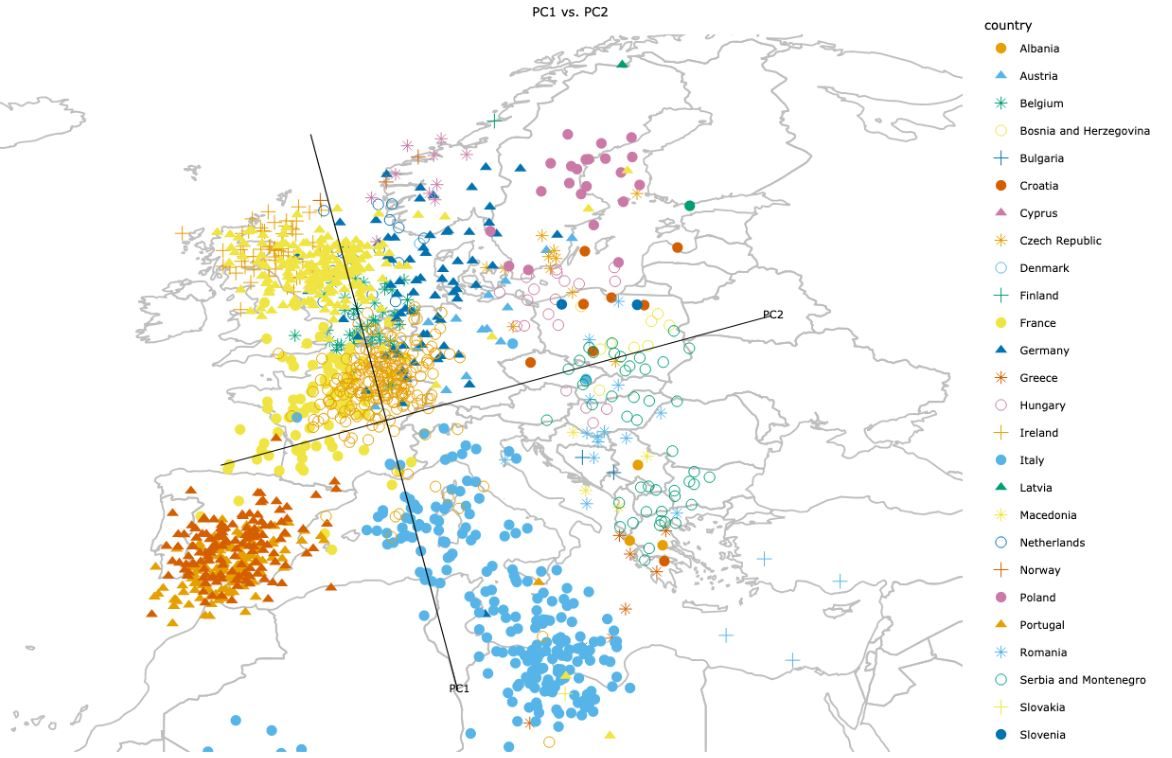
\includegraphics[scale = 0.45]{img/novembre_pca.JPG}
    \caption{An representation of genetic data demonstrating the geographic information contained in European genomes. A simple transformation of genetic data onto two-axes that explain the majority of the genetic variation between populations (i.e. principal components). Recreated using the PCAviz R package. \cite{pcaviz}}
    \label{fig:novembre_pca}
\end{figure}

Genetic information is closely linked to geographic information. Population geneticists have used genetic information to identify historical migration patterns. Computational tools have been developed to estimate migration and highlight features of spatial population structure \cite{petkova_visualizing_2016}. Many early models of spatial evolution assume that populations are discrete and well-mixed \cite{sigwart_coalescent_2009} \cite{kingman_coalescent_1982}, but human genetic data shows continuous spatial structure \cite{novembre_interpreting_2008}. We hope to contribute to spatial population genetics and improve the understanding of the forces that shape population structure.


\section{GWAS and Sampling}
Quantitative and population geneticists are interested in finding statistical associations between genetic variants and particular traits. Recent advances in sequencing technology have enabled large-scale genomic data collection, spawning the "genomics revolution" \cite{lander_initial_2001}. Genome-wide association studies (GWAS) are one common method for detecting associations and are especially useful when attempting to predict an individual’s risk for disease. Disease GWAS function by comparing a large set of genotypes to the known disease trait of members in the group. If members with a particular allele, or variant of a gene, are shown to have a significantly higher probability of also being in the group with the disease, then the GWAS supports the hypothesis that the allele increases one’s risk of developing the disease. GWAS typically estimate the genetic effects on a phenotype by conducting a linear regression as follows \cite{dudbridge_power_2013} \cite{xie_efficiency_1998}:

\begin{equation}
    \hat{\bf{Y}} = \boldsymbol{\hat{\beta}} \bf{G} + \boldsymbol{\epsilon} = \sum_{i=1}^{n} (\hat{\beta_i} G_i + \epsilon_i) 
\end{equation}

Where $\hat{\bf{Y}}$ represents the phenotype expressed as a linear combination of $n$ genetic loci in matrix $\bf{G}$ scaled by their effect sizes $\hat{\beta}$. Error terms are accounted for in $\boldsymbol{\epsilon}$ and are independent from $\bf{G}$. It is important to note that $\hat{\beta}$ is an estimated quantity. Researchers have proposed a number of statistical methods for estimating effect sizes \cite{meuwissen_prediction_2001} \cite{park_distribution_2011}.


With an abundance of genetic information came swathes of analyses and meta-analyses making claims ranging from credible to questionable \cite{ganna_large-scale_2019}. While GWAS have found thousands of statistically significant SNPs associated with particular traits, many criticize geneticists for failing to move beyond identification and into confirmation \cite{visscher_five_2012}. There is, in general, little follow up to confirm how or why a SNP is associated with a trait. Still, many genetic studies have taken the extra step and made meaningful contributions to health and science \cite{belbin_2017}. These include studies that have identified variants for celiac disease and rheumatoid arthritis, respectively and applied these to develop successful tests for individual patients \cite{abraham_accurate_2014} \cite{han_fine_2014}. 


One of the problems with GWAS that we are especially interested in is the issue of sampling bias. GWAS data collection requires researchers to select people to enroll in the study. Due to resource limitations, this selection process is typically restricted to specific populations in specific geographic regions. The vast majority of GWAS study European populations \cite{need_next_2009} \cite{popejoy_genomics_2016} leaving the rest of the world largely in the dark \cite{wojcik_genetic_2019}. 


Population geneticists have previously investigated the effect of geographic sampling bias on theoretical models \cite{mcvean_genealogical_2009}. Some researchers have even shown the effects of sampling bias on distorting population summary statistics like $F_{ST}$ and on simulated GWAS \cite{battey_space_2019}. We hope to expand upon this effort to understand the implications of geographic sampling bias. Our approach to this problem is described in the following section.


\section{Project Rationale and Significance}
Conducting a GWAS requires a large set of genomic data which is gathered by a sampling process. As a result, association studies feature significant geographic sampling bias. For example, the UK BioBank contains samples of people who have migrated to the United Kingdom from around the world, but still represents a small fraction of global diversity \cite{bycroft_uk_2018}. Therefore, it is important to assess if GWAS results from geographically localized studies, such as those from the UK BioBank, can predict disease risk in other geographic regions. This project adds to the existing literature of theoretical models for studying deleterious alleles \cite{eyre-walker_evolution_2010} \cite{pritchard_are_2001}\cite{simons_population_2018}, but is one of the first to consider the influence of spatial sampling bias. The goal of this project is to create a framework for evaluating how geographic sampling bias may affect the detection of rare deleterious alleles. Towards these ends, we note the following aims:	

\begin{enumerate}
    \item Develop a theoretical model to derive the distribution of allele frequencies as a function of the spatial sampling scheme.
    \item Determine the effect of sampling on allele detection probability.
\end{enumerate}


Preliminary studies have shown that deleterious, disease-causing alleles or those with large effects are often rare \cite{marouli_rare_2017} \cite{slatkin_estimating_2000}, and rare alleles are often geographically localized \cite{visscher_r.._2019}\cite{slatkin_spatial_1978}. Through an evolutionary biology lens, we expect deleterious alleles to be removed from a population by natural selection before they can spread far from their location of origin. The rate at which these alleles are removed depends on how deleterious the allele is. Alleles with large deleterious effects are hypothesized to be removed much faster by selection, and therefore be kept rare in a population. As a result, we expect this allele to exist in a relatively small geographic region. Whereas alleles with small effect sizes are expected to span wider regions and exist at higher frequencies. 

\begin{figure}[H]
    \centering
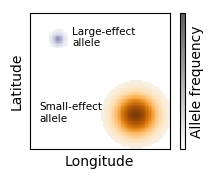
\includegraphics[scale=1.5]{img/spatial_distributions.png}
    \caption{This schematic illustrates the geographic distribution of alleles with varying effect sizes. Large effect, or strongly deleterious alleles are kept at low frequencies and are more geographically isolated due to natural selection. Small effect alleles are found in wider regions and at higher frequencies.}
    \label{fig:spatial_schematic}
\end{figure}


As mentioned previously, GWAS cohorts tend to be geographically localized. This is attributed mostly to convenience and limitations in resources. Researchers do not \textit{yet} have the capacity to sequence all members of a population in all locations, and pooling genomic data from multiple studies may create biased results subject to batch effects \cite{woolston_potential_2015}\cite{gilad_reanalysis_2015}. Therefore, the detection of rare deleterious alleles is especially challenging for GWAS. The ability to detect large-effect alleles is dependent upon process by which researchers sample individuals to sequence. Not only is there a lower probability of sampling individuals with the allele of interest, but small-effect alleles can mask the detection of large-effect alleles. Even if some individuals with the allele of interest are sampled, smaller-effect alleles can comprise a larger proportion of the sample, making large-effect allele detection difficult. There exists a trade-off between sampling individuals in a narrow geographic region, and sampling the same number of people from a broader region. For the former, such a GWAS is more likely to find no associations (landing exclusively in the white space of Figure \ref{fig:spatial_schematic}. While for the latter, such a GWAS may find some of the large-effect allele of interest, but is more likely to not have enough representation in the sample to detect the rare allele. 


A theoretical framework describing the geographic distribution of rare deleterious alleles could help optimize sampling strategies for GWAS cohorts. However, there does not yet exist a framework that considers the interactions between the evolutionary forces acting upon an allele and the sampling process that influences which alleles are detectable. This project aims to construct such a framework. We will utilize population genetic theory and simulations to examine the geographic distribution of rare deleterious alleles. This work is ultimately interested in understanding how the process of sampling may affect the power of a GWAS to detect deleterious alleles. It is predicted that certain sampling schemes may increase the power of a GWAS for certain alleles. The model proposed allows one to quantitatively determine the optimal sampling strategies for given deleterious alleles of varying rarity. This model can ultimately be used to inform future GWAS study design by accounting for sampling effects in data collection, possibly increasing the power of a GWAS to detect rare alleles. This could likely improve GWAS predictions of individual disease risk.